\chapter{Probabiltic Degree Anonymization over Uncertain Graphs}
\label{chp:e}
In this section, we formalize the threat of re-identification combined with the degree probability distributions in the context of uncertain graphs. We study the node degree information incoporates edge uncertainty and show its power to re-identify individual in a uncertain graph. Protecting against the threat of re-identification presents novel challenges for uncertain graph data. Generalization, random perturbation and uncertain graphs methods have been developed for determinitic graph anonymization. It is not trivial to shift these strategies for obfuscating degree probability distributions of nodes in the uncertain graph. 

% waiting for change 
% \section{Naive Approach: Anonymization via Representative Instance}
\label{sec:repOB}
\begin{figure}[t]
    \centering  
        \includegraphics[scale=0.38]{figures/DegreeAUG/repOB.eps}
    	\caption{Illustration of anonymizing an uncertain graph though its representative deterministic instance and its drawback.}
    \label{fig:repOB}
\end{figure}
A naive approach of anonymizing an uncertain graph is to first somehow transform it to a deterministic graph, then perform anonymization processing over the deterministic one. Fortunately, an increasing research effort was dedicated to the topic of exacting representative deterministic graphs from an uncertain graph \cite{Parchas_Gullo_Papadias_Bonchi_2014}. Parchas  {\etal} \cite{Parchas_Gullo_Papadias_Bonchi_2014} ever introduced algorithms for extracting deterministic representative graph which captures key properties of the input uncertain graph. Now, it becomes realizable to anonymize an uncertain graph in two steps as shown in Figure \ref{fig:repOB}. We first extract one deterministic representative instance $G$ from the input uncertain graph $\mathcal{G}$. Then, we anonymize the extracted deterministic graph $G$, and output this result as the anonymized result of the original uncertain graph $\mathcal{G}$ (referred as {\repAn}). 

The {\repAn} approach is attracting since it does not require any new anonymization techniques specific designed for uncertain graphs. When the extracted representative deterministic graph $G$ is close enough to the input uncertain graph $\mathcal{G}$ in terms of graph properties, its anonymized result is expected to be a good anonymization of the input uncertain one. However, there is a non-negotiable difference between the input uncertain graph $\mathcal{G}$ and its deterministic representative instance $G$, as exemplified in Figure \ref{fig:repOB}. The anonymized result of $G$ which is structurally similar to itself instead of the input uncertain graph, consequently, may be far different from the optimal solution, as exemplified in Figure \ref{fig:repOB}. Therefore, we believe that for many applications, the {\repAn} approach,  introducing a high level of noise in such fashion, do reduce the overall graph utility.  In experiment section, we will further illustrate this phenomenon over real-world datasets. 
\section{Probabilitic Degree-based De-anonymization}
In this section, we describe the threat of node re-identification in uncertain graph data, and we explain the content of external information and the use of external information in identifying anonymized individual. We develop the intuition behind achieving anonymity in an uncertain graph through structural similarity to others. 

Here, we remind the reader its difference compared to the deterministic case. The incorporation of uncertainty in the graph data significantly affects the distribution of vertex property. Existing graph perturbation techniques are not equipped to operate over uncertain graphs -- they will tend to ignore and destroy important structural properties. Likewise, uncertain graph structure and adversary knowledge with an incorporation of uncertainty to threaten privacy in new ways. 

\begin{figure}[t!]
    \centering 
    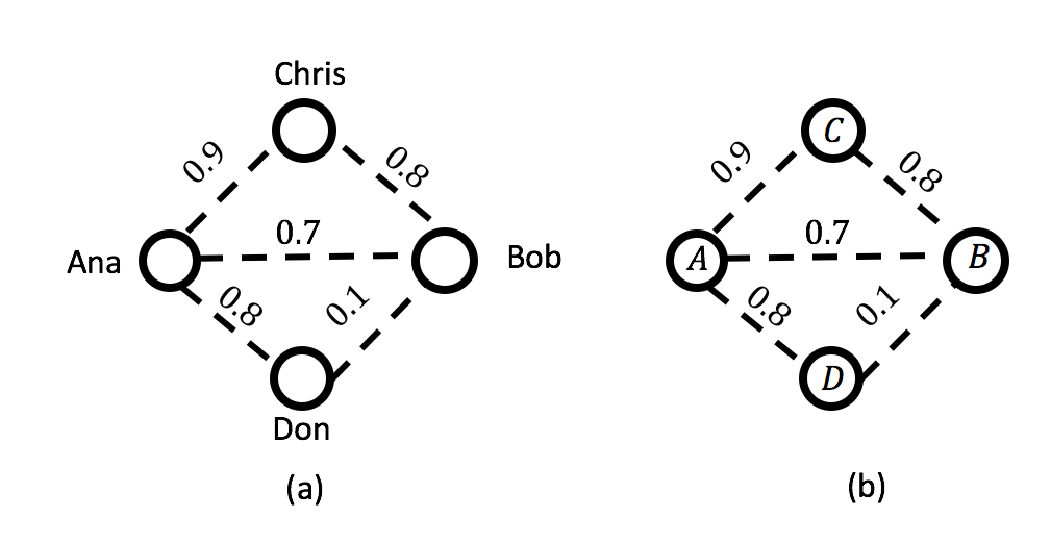
\includegraphics[scale=0.5]{figures/DegreeDistAUG/uncertainExample.eps}
    \caption{\small{(a) The original uncertain graph (b) The naive anonymized version of uncertain graph with 5 edges and $2^{5}=32$ possible world}}
    \label{fig:ddAUG:uncertainGraph}
\end{figure}

To gain more intuition on this attack model and the difficulties in defining a meaningful probabilistic matching, we present a simple example. Consider the original uncertain graph and the anonymized version of the given graph shown in Figure~\ref{fig:ddAUG:uncertainGraph}. We assume the adversary is equipped with the external structural information about some victim nodes. In particular, the property is node degree. Similarly, the degree of any nodes in the anonymized uncertain graph can be expressed as uncertain data. In the case of uncertain graph de-anonymization, the uncertainty belongs to the representation of source objects which are being identified, and the actual assertion is also probabilistic. In other words, fixed the node $v$ in the input uncertain graph, each node $u$ in the anonymized graph has a degree of being the image of $v$, which is probabilistic in nature. Meanwhile, the matching assertion is done by comparing two probability objects. 

\subsection{Adversary Knowledge}
We proceed to present the formal definition. Let us consider the knowledge that an adversary may extract from an uncertain graph about a given target vertex in $\mathcal{G}$. Following the literature, we assume that the adversary knows some vertex property $P$. In this work, we assume such property $P$ is the degree. Given an uncertain graph $\mathcal{G}$, each $v \in \mathcal{G}$ and the degree value $\omega$, we define the probability that $X_{v}(\omega)$ that $v$ originated from a vertex in $G$ with property value $\omega$. Specifically, 
\begin{equation*}
    X_{v}(\omega) = \sum_{G \in W(\mathcal{G})}  Pr(G) \cdot \mathcal{X}_{v,\omega}(G)
\end{equation*}
where $Pr(G)$ is the probability that the possible world $G$ is observed, and $\mathcal{X}_{v,w}(G)$ is 0-1 variable that indicates the vertex $v$ has the degree value $\omega$ in the possible world $G$. In other world, $X_{v}(\omega)$ is the sum of probabilites of all possibel worlds in which the vertex $v$ has the given property value $\omega$. We define the degree value of a node $v$ in an uncertain graph $d_{v}$ as an random variable with a probability distribution $X_{v}$. The probabilties $X_{v}(\omega)$ may be arrange in a $n \times |\Omega|$ matrix, where each row corresponding to one vertex $v in \mathcal{G}$ and it gives the probability distribution $X_{v}$. 
 \begin{table}[t!]
     \centering
      \begin{tabular}{|L{1.25cm}|c|c|c|c|}
             \cline{1-5}
                $\mathbf{X}_{v}(\omega)$ & $\text{deg}=0$ & $\text{deg}=1$ & $\text{deg}=2$ & $\text{deg}=3$ \\ \hline 
              $a$   & $0.006$ & $0.092$ & $0.398$ & $0.504$ \\ 
              $b$   & $0.054$ & $0.348$ & $0.542$ & $0.056$  \\
              $c$   & $0.020$ & $0.260$ & $0.720$ & $0.000$ \\
              $d$   & $0.180$ & $0.740$ & $0.080$ & $0.000$  \\  \hline 
 %              $\mathbf{S(\omega)}$   & $0.260$ & $1.440$ & $1.740$ & $0.560$ \\ \hline 
      \end{tabular} 
      \caption{The matrix $X_{v}(\omega)$ for the uncertain graph in Figure~\ref{fig:ddAUG:uncertainGraph} and the degree property.}
     \label{tab:DegreeMatrix}
 \end{table}


\begin{example}
    Consider the uncertain graph in Figure~\ref{fig:ddAUG:uncertainGraph} and assume the vertex property is degree. Table \ref{tab:DegreeMatrix} gives the corrsponding matrix $X_{v}(\omega)$, in which each row gives the probability distribution regrading the dgree of the corresponding vertex in $\mathcal{G}$. For instance, the probability that $a$ has degree $3$ is $0.9 \cdot 0.7 \cdot 0.8=0.504$. 
\end{example}

\subsection{Re-identification Attack}
The degree value of a node $u$ in the anonymized uncertain graph is defined as the corresponding random variable $d_{u}$.  The matching assertion is evaluated as the probability of the event two random variable $d_{u}$ and $d_{v}$ is equal. Specifically, 
\begin{align*}
    F_{u}(v)=P(d_{u}=d_{v})&=\sum_{\omega} P(d_{u}=\omega) \cdot P(d_{u}=\omega) \\
                  &=\sum_{\omega} X_{v}(\omega) \cdot X_{u}(\omega)
\end{align*}
The probabilities $F_{u}^{v}$ may be arrange in a $n \times n$ matrix, where each row corresponds to one vertex $u \in \tilde{\mathcal{G}}$ and it gives the corresponding probability $F_{u}^{v}$ over all possible target nodes $v \in V_{\mathcal{G}}$. The columns of that matrix are proportional to the probability distribution that correponding to victim nodes. More precisely, the normalized column corresponding to a target node $v$, {\ie}, 
\begin{equation*}
    Y_{v}(u):=\frac{F_{u}(v)}{\sum_{u \in \tilde{G}} F_{u}^{v}}
\end{equation*}
is the probability that $u$ is the image in $\tilde{\mathcal{G}}$ of a vertex that had property $d_{v}$ in $\mathcal{G}$.

 \begin{table}[t!]
     \centering
    \begin{tabular}{|L{1.25cm}|c|c|c|c|}
      \cline{1-5}
      $\mathbf{F_{u}^{v}}}$ & $v_{a}$ & $v_{b}$  & $v_{c}$ & $v_{d}$ \\ \hline 
      $u_{a}$ & 0.42092 & 0.27628 & 0.3106  &  0.101 \\
      $u_{b}$ & 0.27628 & 0.42092 & 0.4818 &  0.3106 \\
      $u_{c}$ & 0.3106  & 0.4818  & 0.5864 &  0.2536 \\
      $u_{d}$ & 0.101   & 0.3106  & 0.2536 &  0.5864 \\  \hline 
    \end{tabular}
    \caption{The matrix $F_{u}^{v}$ for the uncertain graph and itself in Figure~\ref{fig:ddAUG:uncertainGraph} and the degree property.}
    \label{tab:DegreeDistMatching}
 \end{table}


 \begin{table}[t!]
     \centering
    \begin{tabular}{|L{1.25cm}|c|c|c|c|}
      \cline{1-5}
      $\mathbf{Y_{u}^{v}}}$ & $v_{a}$ & $v_{b}$  & $v_{c}$ & $v_{d}$ \\ \hline 
      $u_{a}$ & 0.37962     & 0.18548  & 0.19027  &  0.08069 \\
      $u_{b}$ & 0.24917     & 0.28257  & 0.29515  &  0.24816 \\
      $u_{c}$ & 0.28012     & 0.32344  & 0.35922  &  0.20262 \\
      $u_{d}$ & 0.09109     & 0.20851  & 0.15535  &  0.46852 \\  \hline 
    \end{tabular}
    \caption{The matrix $Y_{u}^{v}$ for the uncertain graph and itself in Figure~\ref{fig:ddAUG:uncertainGraph} and the degree property.}
    \label{tab:DegreeDistPreimage}
 \end{table}

\begin{example}
    For example, if in the anonymization process we do nothing, then the perturbed output $\tilde{\mathcal{G}}=1$. In the case, the probability matrix induced by $\tilde{\mathcal{G}}$ equals to the one induced by $\mathcal{G}$. Table \ref{tab:DegreeDistMatching} gives the corresponding matrix $F$. For instance, the probability that $d_{a}$ is equal to $d_{c}$ is $0.006 \cdot 0.02 + 0.092 \cdot 0.26 + 0.398 \cdot 0.72 + 0.504 \cdot 0=0.3106$. After normalization them, give the corresponding $Y_{u}(v)$  distributions for each vertex $v$ in Table \ref{tab:DegreeDistPreimage}. For instance, if we look for a vertex that has the same degree distribution of $Ana$ in $\mathcal{G}$, it is either $a$, with probability around $0.38$, $b$ with probability around $0.25$, $c$ with probability around $0.28$, or $d$ with probability around $0.09$. 
\end{example}

\subsection{Privacy Notation}
Likewise, we can define our notion of privacy . 
\begin{definition}
    \textbf{\boldmath{$(k,\epsilon)$}-obf \cite{Bonchi_Identity_2014}}
    Let $P$ be the degree distribution, $k \geq 1$ be a desired level of anonymity, and $\epsilon >0 $ be a tolerance parameter. The uncertain graph $\tilde{\mathcal{G}}$ is said to $k$-obfuscate a given vertex $v \in V_{\mathcal{G}}$ with respect to $P$ if the entropy of the distribution $Y_{v}$ over the vertices of $\mathcal{G}$ is greater than or equals to $\log_{2}{k}$:
    \vj
    \begin{equation*}
        H(Y_{v}) \geq \log_{2}{k}.
    \label{obfCon}
    \svj
    \end{equation*}
The uncertain graph $\mathcal{G}$ is $(k,\epsilon)$-obf with respect to property $P$ if it $k$-obfuscates at least $(1-\epsilon)|V|$ vertices in $V_{\mathcal{G}}$. $P$ can be any node properties.  
\end{definition}
Namely, given the considered attack scenario, in which the adversary uses the degree distribution information of his target vertex $v$, we wish to lower bound the entropy of the distribution it induced over the perturbed graph vertices by $\log_{2}{k}$. The general idea is exact the same with {\keobf}, proposed in the literture~\cite{Bonchi_Identity_2014}. We extend the concept of equivalent class to probabilitic scenerio. 
\section{Probabilitic Degree Anonymization}
The uncertainty injecting scheme resembles the degree anonymization method designed for the deterministic graph. One common heuristics is to select the perturbation budget for each selected edge $e=(u,v)$, depending on properties of  the vertices $u$ and $v$. The perturbation will be larger for edges that connect unique vertices, which, require higher levels of uncertainty to ``blend in the crowd", and smaller for edges that connect more ``typical" vertices. Note that, it requires one effective method to capture how typical a given vertex is among all the vertices in the uncertain graph, in terms of vertex property $P$. In this work, let us consider vertex property $P$ be node degree. In this case, namely, it is related to cluster uncertain data (distribution). The key feature of our method is to incorporate the statistical distance function for calculating the uniqueness level of vertices with regards to their node degree. 

\subsection{Uniqueness Score of Vertices}
\begin{figure*}[t!]
     \begin{subfigure}[b]{1\textwidth}
        \centering
        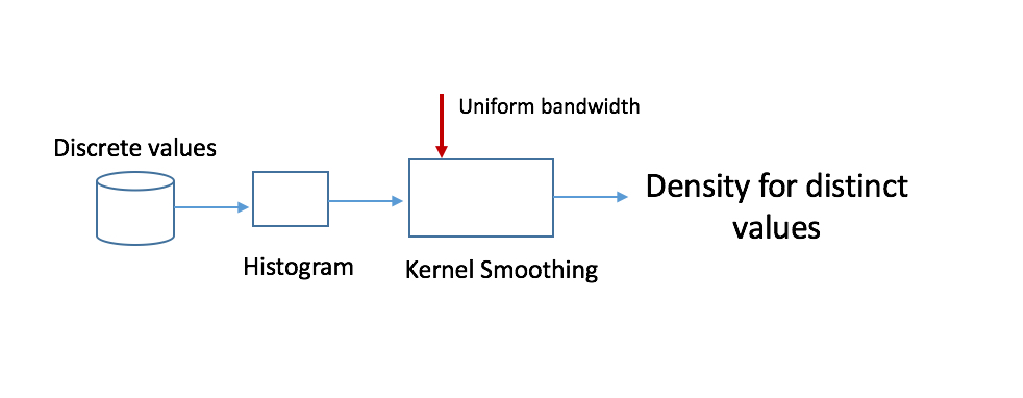
\includegraphics[scale=0.7]{figures/DegreeDistAUG/uniqueD.eps}
        \caption{Density estimation of nodes degree (Determinitic cases)}}
        \label{fig:uniqueDcal}
    \end{subfigure}%
    \begin{subfigure}[b]{1\textwidth}
		\centering
        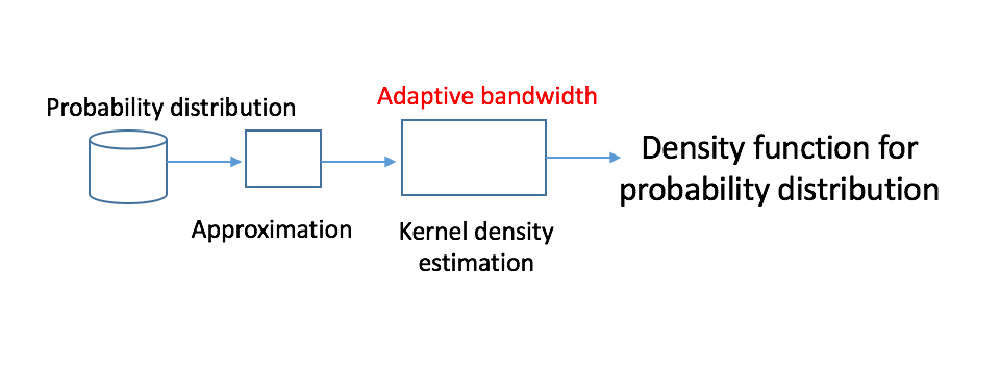
\includegraphics[scale=0.7]{figures/DegreeDistAUG/uniqueDD.eps}
        \caption{Density estimation of nodes degree (Uncertain cases)}}
        \label{fig:uniqueDDcal}
    \end{subfigure} 
    \caption{Comparison of determinitic and uncertain vertex density estimation in terms of node degree.}
\end{figure*}
For vertex properties of interest, such as degree, the majority of vertices in the real uncertain graphs are already anonymous even without random perturbation. The phenomena inherit from the one in the deterministic graph. The majority of vertices in the graph have a low degree ($\le 10$) with quite similar distribution. Hence, we aim at controlling the amount of applied perturbation, so that larger perturbation is added at vertices that are less anonymized in the original graph, namely, outlier point with respects to its degree distribution. In particular, we suggest calibrating the perturbation applied to an edge $e=(u,v) \in E_{c}$ according to the ``uniqueness" of the two vertices $u$ and $v$ with respect to the property $P$. Namely, if both $P(u)$ and $P(v)$ are in the dense region, then $r_{e}$ should be very small; on the other hand, if $P(u)$ and $P(v)$ are outlier values, then $r_{e}$ should be higher. The definition is quite similar to the ``uniqueness score", proposed in~\cite{} while extended for dealing with uncertain objects. 

Let $P$: $V \rightarrow \Omega$ be node degree defined on the set of vertices $V$ in an uncertain graph. Clearly, $\omega$ denotes uncertain object (random variable). Further, consider a distance function $d$ between  random variables in the range $\Omega$. So, for each pair of random variables,$p$ and $q$, distance $d(p,q) \ge 0$ is defined. For the degree property $P_{1}$, a natural candidate of statistical distance function is Bhattacharyya distance. For probability distribution $p$ and $q$ over the same domain $X$, the Bhattacharyya distance is defined as: 
\begin{equation*}
    D_{B}(p,q)=-ln(\sum_{x} \sqrt{p(x) \cdot q(x)})
\end{equation*}
Before the computing of statistical distance between probability distributions, we need to get the probability distribution for all the vertices in the uncertain graph. The probability distribution of $d_{v}$ may be computed exactly in time $O(n^2)$ or be approximated in time $O(n)$. The statistical distance between two probability distribution may be computed exactly in time $O(n)$. The overall complexity is $O(n^{3})$. Clearly, it is not suitable for large uncertain graphs. Note that, the uniqueness function is used for locating outlier points. For the degree property, they are nodes with high degree. In such case, we may adopt an alternative approach. Since the $d_{v}$ is the sum of independent random variable, it may be approximated by the normal distribution $N(\mu, \sigma^{2})$, where $\mu= \sum p_{e_i}$  and $\sigma^2= \sum p_{e_i} \cdot (1-p_{e_{i}})$ as implied by the Central Limit Theorem. The Central Limit Theorem becomes effective already for $n \approx 30$. For typicals size of $n$ in large uncertain graphs, the normal approximation becomes very accurate. According to the normal approximation, the Bhattacharyya distance between two normal distribution can be cacluated~\cite{} by exacting the mean and variances of two separate distribution objects: 
\begin{equation*}
    D_{B}(p,q)=\frac{1}{4} \cdot \ln{\frac{1}{4} 
                (\frac{\sigma_{p}^2}{\sigma_{q}^2} + \frac{\sigma_{q}^2}{\sigma_{p}^2}+2)}+
                \frac{1}{4} \cdot (\frac{(\mu_{p}-\mu_{q})^{2}}{\sigma_{p}^2+ \sigma_{q}^2})
\end{equation*} 
By this way, we map the object (probability distribution) from high dimension to 2D space. It speed up the computation of ``uniqueness score''. The overall time complexity is $O(n^2)$ where $n$ is the number of vertices in the uncertain graph. The quartic complexity is not suitable for dealing with large networks. 

Note that, the definition of the uniquness score is related to the kernel density estimation. For the specific method proposed in the literture~\cite{Boldi_Injecting_2012}, it adopts the gaussian function as a weighting function (kernel), the absolute difference as a distance function and the parameter $\theta$ for setting bandwidth. H
For computing the distance between probability distributions, the statistical distance functions were choosed. The remaining issue is the choice of bandwidth. Note that, the choice of bandwidth has the siginificant effect on the shape of the corresponding kernel density estimator. If the bandwidth is small, we will obtain an under smoothed estimator, with high variability. On the contrary, if the value of bandwidth $h$ is big, the resulting estimator will be over smooth and farther from the real data distribution that we are trying to estimate. Notice of the connection between uniqueness and density estimation, we adopt the adaptive bandwidth kernel density estimation method, {\ie}, we vary the w of the kernel in different regions of the sample space. By this way, we can get the statistical robust estimation of the distribution of all the vertices in the input uncertain graph in an efficient way. 

\subsection{Proposed Research Tasks}
\begin{itemize}
    \item {We identify and formulate the node re-identification attack using their degree probability distribution, and extend the {\keobf} notation for quantifying privacy level. We present the reliability and privacy preserving problem in the context of uncertain graphs.}
    \item {We show case that a naive approach that simply combines existing techniques do not work in practice due to significant utility loss.}
    \item {We propose a heuristic based on the density estimation of probability distributions among all the vertices in the uncertain graph for injecting perturbation judiciously. We give an efficient and effective method for heuristic evaluation.}
    \item {We propose to explore different search strategy for solving the induced optimized problem in the process of injecting uncertainty. }
    \item {We perform an extensive experimental evaluation using four real-world uncertain graph data sets from different  domains. We evaluate and compare our methods using different groups of graph metrics.}
\end{itemize}